\chapter{Asking Millionaires How They Got RICH! (Houston)}

This chapter follows a School of Hard Knocks field interview in Houston, curated by LazyingArt LLC. The source is not a blackboard lecture, but it still unfolds with a real quantitative logic. Again and again we are asked to separate yearly income from asset value, disciplined saving from scaled capital, labor from leverage, and wealth creation from wealth preservation. The opening montage advertises extreme outcomes; the body of the lecture tries, case by case, to tell us what mechanism sits behind them.

\section{Houston as a Wealth Field}

The lecture begins with a preview reel cut from later moments: the most amount of money made in a year, industrial real estate, champagne, Lamborghinis, and Houston's high millionaire density. This is not yet argument. It is a staging device. We are shown the prizes first so that the later interviews can answer the real question: what habits, structures, and decisions could plausibly generate outcomes of that scale?

The first discipline the notes must impose is accounting. The host asks in ordinary language how much money someone made in a year, but the respondents often answer in a mixed language of salary, business scale, portfolio value, and social position. If we do not separate those categories, the rest of the lecture dissolves into glamour. We therefore keep three quantities in view: yearly realized earnings \(Y_{\mathrm{annual}}\), accumulated wealth \(W_t\), and portfolio value \(P\).

\begin{equation}
Y_{\mathrm{annual}} \not\equiv P,
\qquad
P = \sum_j V_j.
\end{equation}

This first distinction does a great deal of work. It tells us how to hear the montage. Some of the biggest numbers in the lecture are not wage income at all, but marked values of held assets. The host then narrows from spectacle to fieldwork: Houston is the setting, and the day's project is to ask wealthy people directly how they became wealthy. We have our laboratory.

\section{First Anchor Case: Leadership, Foundation, and Early Saving}

The first sustained interview is deliberately sober. The speaker does not begin with toys or status symbols. He says he runs a company, solves a lot of problems, and leads an insurance brokerage firm described as a multi-billion-dollar company. The tone matters. Before the lecture becomes numerical, it first becomes operational.

\paragraph{Anecdote.} The interview begins with business identity and scale. It then turns backward: what would one tell the younger self at the beginning?

\paragraph{Claim.} ``Be bold'' is the memorable phrase, but the next sentence is the real correction. Get some education behind you. Get some foundation. Young people want to make it fast; the speaker insists on four or five years of understanding one's discipline before striking out independently.

\paragraph{Mechanism.} The lecture refuses to treat success as mere appetite. It puts apprenticeship before acceleration. That prepares the move into finance proper.

The financial advice is concrete. Read foundational personal-finance books, save money early, and use the spoken ``rule of seven'' as a compounding heuristic. The transcript never defines that heuristic precisely, so we keep the mathematics modest and explicit about its status. The cleanest reconstruction is a standard accumulation rule:

\begin{equation}
W_{t+1} = (1+r)W_t + sY_t,
\end{equation}

where \(W_t\) is wealth at time \(t\), \(Y_t\) is annual income, \(s\) is the savings rate, and \(r\) is an implied rate of return introduced only to express the idea of compounding.

The speaker also supplies a concrete band for the savings rate and a concrete income bracket for the example he has in mind:

\begin{equation}
s \in [0.10,\,0.20],
\qquad
Y \in [70{,}000,\,80{,}000]\ \text{dollars per year}.
\end{equation}

The lecture's claim is then that this discipline can produce millionaire status by roughly age thirty or forty, even on those earnings, and the same speaker says he himself first became a millionaire at twenty-eight. The source does not prove the claim line by line, but it unmistakably presents it as a mechanism claim rather than as a motivational slogan.

\subsection{Question \& Answer}

\paragraph{Question.} How does ordinary earnings turn into wealth?

\paragraph{Answer.} The answer given here is repetitive accumulation. Save a stable fraction of income, begin early, and let time work on the stock rather than spending everything in the present.

A cautious worked example makes the point. Take an annual income in the middle of the speaker's range and a mid-band savings rate:
\begin{align}
Y &= 75{,}000,\\
s &= 0.15.
\end{align}
Then yearly saving is
\begin{equation}
sY = 11{,}250.
\end{equation}

If we interpret the spoken ``rule of seven'' only as a rough doubling heuristic, then the lecture's intuition may be summarized by
\begin{equation}
W(t+7) \approx 2W(t).
\end{equation}
We should not treat this as an exact law. The point is structural. Early dollars have more time to be transformed by repeated growth than late dollars do.

The logic can therefore be written in a short sequence:
\begin{enumerate}
\item Start from yearly cash income \(Y\).
\item Save a fixed fraction \(s\), producing yearly contribution \(sY\).
\item Add that contribution to the accumulated stock \(W_t\).
\item Repeat the process over many years.
\item Let compounding work on the stock rather than consuming it immediately.
\end{enumerate}

The interview then pivots, and the pivot matters. After money comes philanthropy: helping people, giving money away, and speaking of success in terms of changing lives. The exact legal meaning of ``501c'' is not developed in the transcript, so we do not overformalize it. But the structural move is clear. Wealth is not left standing as a pile of private gain. It is immediately reframed as stewardship.

\section{Second Anchor Case: Portfolio Logic, Concentrated Risk, and Marketing}

The host now says, in effect, let us go again. We are moved to a wealthy restaurant district in Houston, told of a promising table, told to come back in ten minutes, and then dropped into the lecture's sharpest wealth-mechanics case. The preview montage now begins to cash itself out.

\paragraph{Anecdote.} The speaker starts in oil and gas, studies at TCU and Rice, works as a project manager, becomes an angel investor, has several successful exits, and then starts a private equity firm.

\paragraph{Claim.} Wealth at this scale is no longer described chiefly as salary. It is described as position, holdings, and capital allocation.

\paragraph{Mechanism.} The path is sequential: salary labor becomes early-stage investing, early-stage investing produces exits, exits produce a platform, and the platform produces a portfolio.

\begin{figure}[h]
\centering
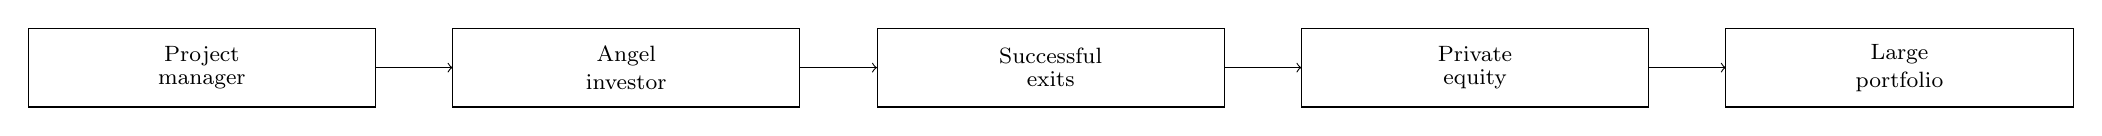
\begin{tikzpicture}[x=2.45cm,y=1.25cm]
\draw (0,0) rectangle (1.8,0.8);
\node at (0.9,0.4) {\shortstack{\footnotesize Project\\\footnotesize manager}};
\draw (2.2,0) rectangle (4.0,0.8);
\node at (3.1,0.4) {\shortstack{\footnotesize Angel\\\footnotesize investor}};
\draw (4.4,0) rectangle (6.2,0.8);
\node at (5.3,0.4) {\shortstack{\footnotesize Successful\\\footnotesize exits}};
\draw (6.6,0) rectangle (8.4,0.8);
\node at (7.5,0.4) {\shortstack{\footnotesize Private\\\footnotesize equity}};
\draw (8.8,0) rectangle (10.6,0.8);
\node at (9.7,0.4) {\shortstack{\footnotesize Large\\\footnotesize portfolio}};
\draw[->] (1.8,0.4) -- (2.2,0.4);
\draw[->] (4.0,0.4) -- (4.4,0.4);
\draw[->] (6.2,0.4) -- (6.6,0.4);
\draw[->] (8.4,0.4) -- (8.8,0.4);
\end{tikzpicture}
\end{figure}

The key exchange arrives when the host asks for the most amount of money made in a single year. The respondent does not answer with salary, and not even cleanly with distributions. He says, first, ``Portfolio range, about 420,'' and then, when pressed, clarifies that the number is \(420\) million.

\begin{equation}
P \approx \$420\,\text{million}.
\end{equation}

Later the host paraphrases the number as a portfolio valued at over \(400\) million. The precise valuation convention is never given, but the essential lesson is plain: the answer is a stock answer to a flow question.

\subsection{Question \& Answer}

\paragraph{Question.} What does ``money made in a year'' mean when wealth sits in assets?

\paragraph{Answer.} In this segment it means, at best, something mixed. The interviewer asks for annual gain, but the respondent explicitly pivots away from dividends and toward portfolio value. Once wealth becomes asset-heavy, annual position may be expressed in marked holdings rather than in wage or salary income.

That is why this distinction has to remain active:
\begin{equation}
Y_{\mathrm{annual}} \not\equiv P.
\end{equation}

The interview does not build a valuation model, and we should not smuggle one in. But it does force a conceptual correction. Large wealth often appears to the outside observer as ``what someone made,'' when the relevant quantity is really ``what someone holds.''

Once that clarification is made, the lecture pushes immediately toward risk. Snapchat is named as the largest risk in the career. The speaker says the seed-round ask was about \(20{,}000\) dollars, at a time when salary was about \(80{,}000\) dollars. So the risk fraction is straightforward:

\begin{equation}
\frac{I_{\mathrm{Snap}}}{Y_{\mathrm{salary}}}
=
\frac{20{,}000}{80{,}000}
\approx 0.25.
\end{equation}

This is one of the cleanest numerical moments in the lecture. The choice was not merely ``bold.'' It amounted to placing roughly one quarter of annual salary into one early-stage opportunity.

The later payoff is described as approximately \(\$72\) million from Snap and the other companies in the portfolio. Because the transcript fuses a single investment with the larger portfolio, we preserve the number but resist over-cleaning the algebra. What matters is the asymmetry: relatively ordinary salary on the way in, extraordinary upside on the way out.

The next question asks what takes a business from seven figures to eight and nine. The answer is immediate: marketing. Not as ornament, but as scale variable. The source's language is rough, but the mechanism is clear. Proper marketing increases reach; increased reach widens the population of buyers or investors; wider reach is what turns a small success into a large one. The lecture is not saying that product quality is irrelevant. It is saying that distribution governs scale.

The final move in this case is from creation to preservation. The respondent's advice is to find loopholes, buy assets under separate entities, lease to oneself, and capture write-offs. The notes should preserve the logic while staying cautious about its legal status: once wealth has been created, structure determines how much of it stays in hand.

\section{From Networks to Operating Rules}

The host now steps in to interpret what has just happened. This commentary is easy to dismiss, but we should not dismiss it. The host's summary is the lecture's way of turning anecdote into mechanism. The large portfolio is not explained as magic. It is explained as access: connections, rooms, deals, and the ability to move among people wealthier than oneself.

There is an important shift here. We are no longer only talking about capital. We are talking about social capital. The host's recap says, in effect, that some fortunes are built not only by selecting assets well, but by standing close enough to the right people and opportunities that one can even see those assets in time.

The next speaker compresses this logic further with a phrase remembered from youth: \(90\%\) of success is showing up. We should not read the number as a measured coefficient. Its role in the lecture is heuristic. The claim is that reliability creates trust, and trust turns into opportunity. This is followed by one of the lecture's sharpest reductions: most people, when they invest, do not invest in businesses; they invest in people.

That line could easily become slogan if left alone. The lecture rescues it by moving immediately to a service-business example. A restaurant owner says the biggest differentiator is details: remembering children's names, birthdays, cakes, handwritten notes, the small acts that turn a transaction into remembered care. The point is not sentimentality. It is operational differentiation. Details are how trust is made concrete.

There is also a brief social-proof interlude in which a prior interviewee reports that \(150\) to \(200\) people approached him after an earlier video. That moment is not mathematically deep, but it does fit the lecture's logic: reputation compounds too. Visibility, repeated appearance, and recognizability are treated as assets in their own right.

By now the lecture has distilled several portable rules:
\begin{itemize}
\item show up consistently enough that others can rely on you;
\item understand that capital often follows trust;
\item make trust legible through details, follow-through, and care;
\item treat relationships as infrastructure rather than as decoration.
\end{itemize}

\section{Case Cluster: Aspiration, Decisions, Sales, and Niche Strategy}

The last movement of the chapter broadens the field. Instead of one long case, we are given a sequence of smaller tests. The question is no longer whether the same rule holds in one industry; it is whether the underlying logic survives across very different kinds of work.

A Lamborghini owner offers the purest aspiration claim in the lecture: put it out into the universe, visualize it, go after it, and do not give up. Taken by itself, this is too loose to bear much analytic weight. But the lecture does not leave it by itself. The host immediately ties the encounter back to restaurant ownership and value creation. Desire remains in the picture, but it is pressed back toward execution.

The engineering interview supplies a stronger conceptual metaphor. The speaker imagines life as a ledger of numbered decisions, with early decisions carrying especially large downstream effects. This is not a literal equation from the source, but it is a useful transcript-based schematic of path dependence: good early decisions widen later options, while bad early decisions constrain and compound into future difficulty.

\begin{figure}[h]
\centering
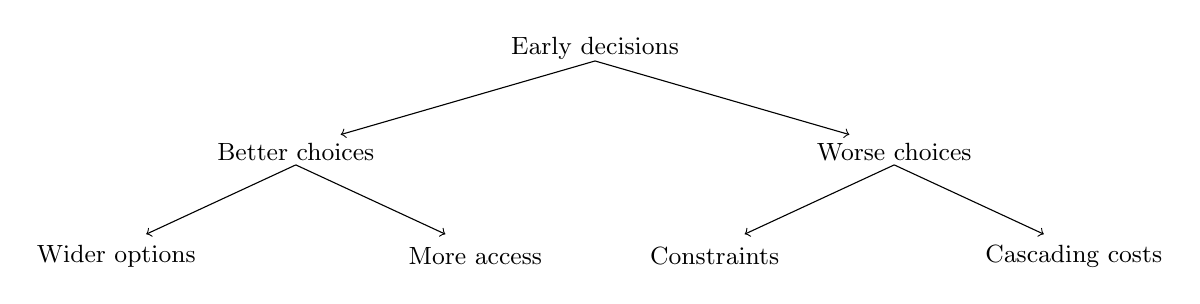
\begin{tikzpicture}[x=1.9cm,y=1.1cm]
\node at (0,0) {\small Early decisions};
\node at (-2,-1.2) {\small Better choices};
\node at (2,-1.2) {\small Worse choices};
\node at (-3.2,-2.4) {\small Wider options};
\node at (-0.8,-2.4) {\small More access};
\node at (0.8,-2.4) {\small Constraints};
\node at (3.2,-2.4) {\small Cascading costs};
\draw[->] (0,-0.15) -- (-1.7,-1.0);
\draw[->] (0,-0.15) -- (1.7,-1.0);
\draw[->] (-2,-1.35) -- (-3.0,-2.15);
\draw[->] (-2,-1.35) -- (-1.0,-2.15);
\draw[->] (2,-1.35) -- (1.0,-2.15);
\draw[->] (2,-1.35) -- (3.0,-2.15);
\end{tikzpicture}
\end{figure}

Industrial real estate returns us to blunt operating language. The company buys, builds, and leases large industrial properties across the country. The most annual amount made is said to be over a million dollars. The scaling rule is plain:

\begin{equation}
H \approx 60\ \text{hours/week}.
\end{equation}

The associated sales rule is equally plain: listen. Do not monopolize the conversation; understand needs and wants; then close the deal. The lecture repeatedly turns large outcomes back into repeatable habits.

The renewable-energy marketing interview restates the distribution theme in a new idiom. The business is social-media marketing, but the secret of strong brand-building is said to lie outside the platforms themselves, in networking and relationship-building. The annual income claim is also concrete:

\begin{equation}
Y_{\mathrm{renewable}} \approx \$350{,}000 \text{ to } \$500{,}000.
\end{equation}

The associated financial advice is to save early and use real estate as part of the investment path, though the transcript in this section becomes repetitive and unstable.

The REIT segment is more corrupted still, but one number survives cleanly:

\begin{equation}
D_{\mathrm{REIT}} \approx \$1.2\,\text{million}.
\end{equation}

The deeper point is qualitative rather than numerical. The speaker insists that the value of the deal is not exhausted by cash up front. Tax breaks, structure, and side benefits matter as well. That keeps intact one of the lecture's recurring distinctions: nominal scale and effective retained value are not the same thing.

The final case, in the champagne business, circles back to a theme we have now heard in several forms. Passion may start the enterprise, but only study, positioning, and execution sustain it. The speaker describes years of exposure, travel, product learning, and then the hard questions of market, competition, price point, margins, and contingencies. Even here, at the lecture's end, the same form persists. Aspiration alone is never left alone; it is always put back under discipline.

\section{Summary}

The Houston lecture does not yield a single master formula for wealth. What it offers instead is a layered model, disclosed in the order the interviews make it available. First we are shown the scale of the outcomes. Then we learn to separate yearly cash flow from portfolio value. Then we are given disciplined saving and compounding, followed by concentrated risk, marketing as a lever of scale, entity structure as a mode of preservation, and trust as the medium through which opportunities are seen and taken.

The chapter's underlying distinctions are therefore simple but decisive. Salary is not portfolio. Boldness is not enough without formation. Growth is not the same as retention. Visibility is not the same as value, though it can help create value. And relationships are not a decorative side theme; they are one of the lecture's main mechanisms of entry into larger rooms and larger deals.

The source is informal, sometimes jagged, and occasionally garbled, but the lecture still unfolds step by step. First discipline, then leverage; first credibility, then access; first creation, then preservation. That is the mathematical and commercial spine of the chapter, and it is enough to make the sequence coherent without forcing the material into a theorem it never claimed to prove.